\begin{figure}[!htb]
\setlength{\unitlength}{\textwidth}

  \begin{picture}(1,0.38)(0,0.74)
    
  \put(0.4,0.76){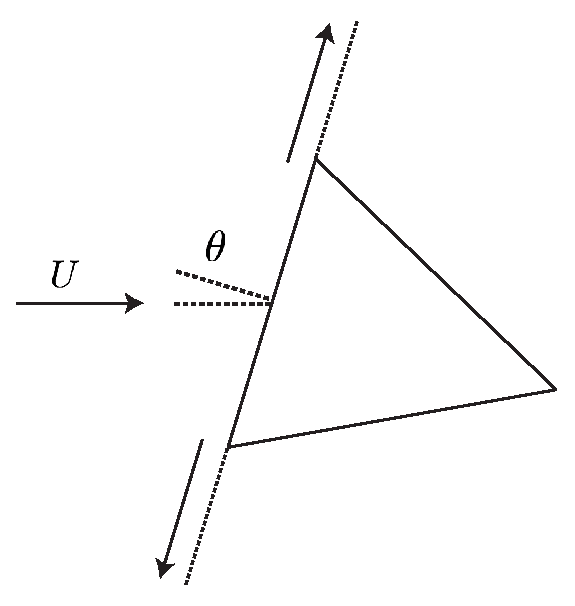
\includegraphics[width=0.25\unitlength]{./chapter-cross-sections/fnp/tri-sketch.eps}}         
      
      
   
 	\put(0.38,0.937){$\theta$}
 	%\put(0.52,0.74){$l$}
   

 	
 	 

     

  \end{picture}

 \caption{Illustration of the lines along which the flow velocity magnitudes have been extracted. The data have been extracted along a line starting from the separation points in the outward direction (shown with arrows) for the top and bottom surfaces.}
    \label{fig:tri-sketch}
\end{figure}